\subsection{Years of Battles per Countries}
In Figure \ref{fig:FightingDurationRanking}, we observe that among all the countries, the United States are the one that fought the most. The second country in this ranking is the Ottoman Empire with only 14 years, which is less than half the number of years that the USA spent in war.
 \begin{figure}[h]
	\centering	\includegraphics[width=0.5\textwidth]{figures/YearsFightingRanking}
	\caption{Years in which the United States were engaged in a battle for at least 1 day.}\label{fig:FightingDurationRanking}
	\centering
\end{figure}

These results tend to support the common belief that the United States are always in war. In fact, they proclaimed their independence in 1776 and have been engaged in at least one battle each year for more than 145 years in total during their 242 years of existence. In Figure \ref{fig:USAFightingTimeline}, we show that even though the United States have almost never stop fighting and also observe that since 2000, the USA are continually engaged in battles.
 
 \begin{figure}[h]
 	\centering	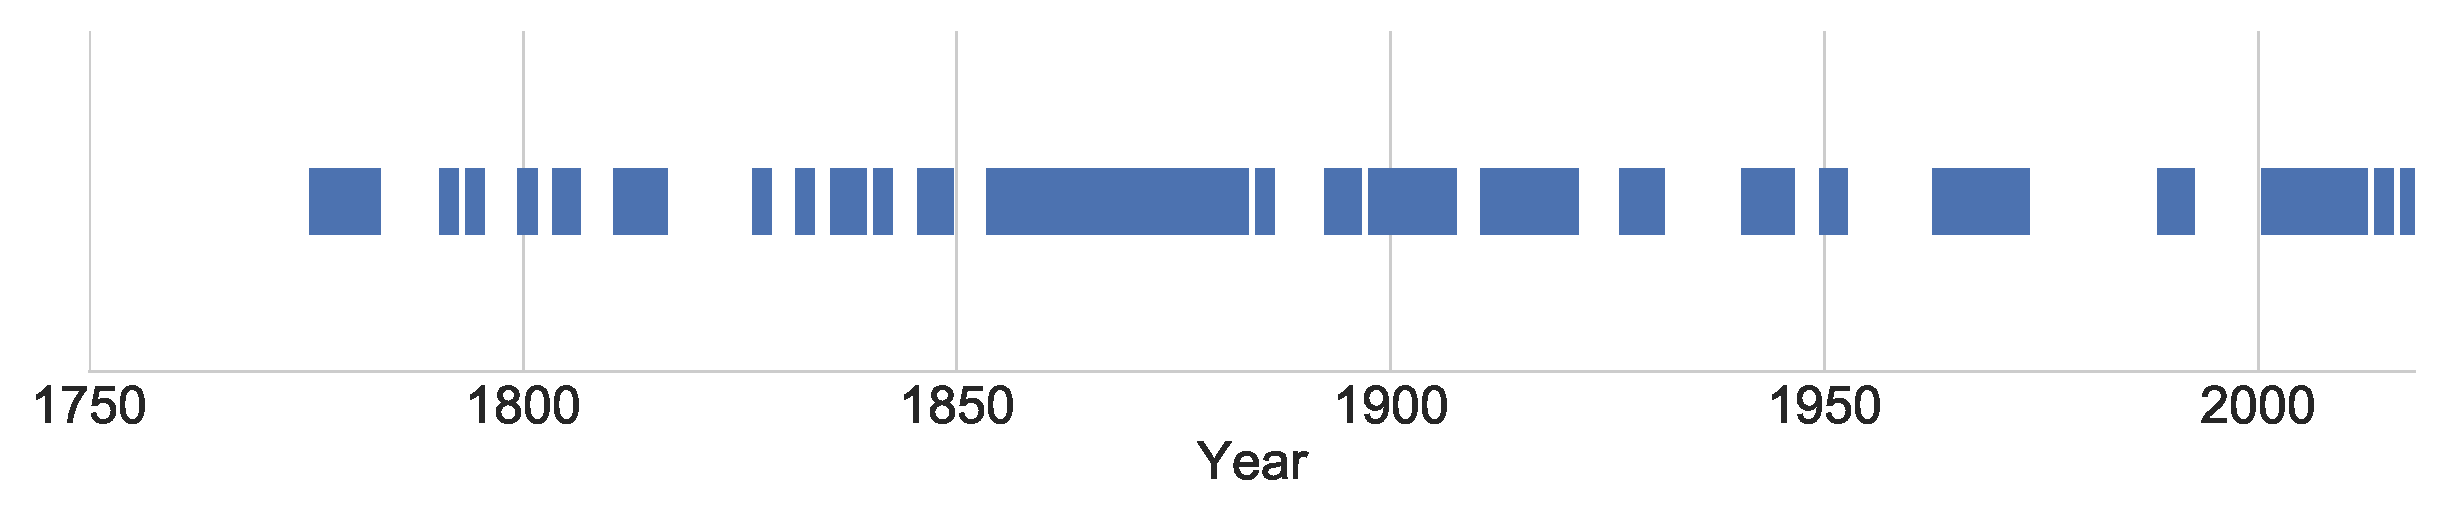
\includegraphics[width=0.5\textwidth]{figures/USAFighting}
 	\caption{Timeline of the USA engagement in battles.}\label{fig:USAFightingTimeline}
 	\centering
 \end{figure}

 